% Created by tikzDevice version 0.12.6 on 2025-07-29 11:45:13
% !TEX encoding = UTF-8 Unicode
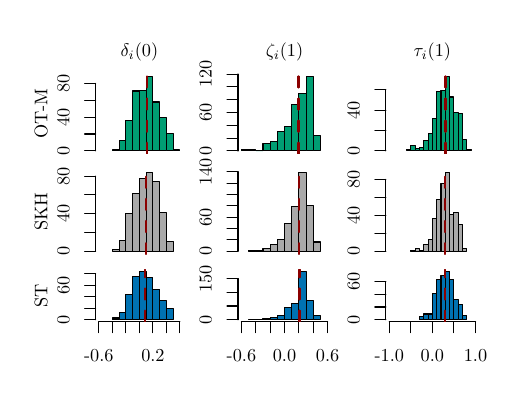
\begin{tikzpicture}[x=1pt,y=1pt]
\definecolor{fillColor}{RGB}{255,255,255}
\path[use as bounding box,fill=fillColor,fill opacity=0.00] (0,0) rectangle (166.22,122.86);
\begin{scope}
\path[clip] ( 24.55, 77.26) rectangle ( 56.20,106.23);
\definecolor{drawColor}{RGB}{0,0,0}
\definecolor{fillColor}{RGB}{0,158,115}

\path[draw=drawColor,line width= 0.4pt,line join=round,line cap=round,fill=fillColor] ( 30.61, 78.33) rectangle ( 33.05, 78.64);

\path[draw=drawColor,line width= 0.4pt,line join=round,line cap=round,fill=fillColor] ( 33.05, 78.33) rectangle ( 35.49, 81.99);

\path[draw=drawColor,line width= 0.4pt,line join=round,line cap=round,fill=fillColor] ( 35.49, 78.33) rectangle ( 37.93, 89.30);

\path[draw=drawColor,line width= 0.4pt,line join=round,line cap=round,fill=fillColor] ( 37.93, 78.33) rectangle ( 40.37, 99.97);

\path[draw=drawColor,line width= 0.4pt,line join=round,line cap=round,fill=fillColor] ( 40.37, 78.33) rectangle ( 42.82,100.28);

\path[draw=drawColor,line width= 0.4pt,line join=round,line cap=round,fill=fillColor] ( 42.82, 78.33) rectangle ( 45.26,105.15);

\path[draw=drawColor,line width= 0.4pt,line join=round,line cap=round,fill=fillColor] ( 45.26, 78.33) rectangle ( 47.70, 96.01);

\path[draw=drawColor,line width= 0.4pt,line join=round,line cap=round,fill=fillColor] ( 47.70, 78.33) rectangle ( 50.14, 90.52);

\path[draw=drawColor,line width= 0.4pt,line join=round,line cap=round,fill=fillColor] ( 50.14, 78.33) rectangle ( 52.58, 84.73);

\path[draw=drawColor,line width= 0.4pt,line join=round,line cap=round,fill=fillColor] ( 52.58, 78.33) rectangle ( 55.02, 78.64);
\end{scope}
\begin{scope}
\path[clip] (  0.00,  0.00) rectangle (166.22,122.86);
\definecolor{drawColor}{RGB}{0,0,0}

\path[draw=drawColor,line width= 0.4pt,line join=round,line cap=round] ( 24.55, 78.33) -- ( 24.55,102.72);

\path[draw=drawColor,line width= 0.4pt,line join=round,line cap=round] ( 24.55, 78.33) -- ( 20.59, 78.33);

\path[draw=drawColor,line width= 0.4pt,line join=round,line cap=round] ( 24.55, 84.43) -- ( 20.59, 84.43);

\path[draw=drawColor,line width= 0.4pt,line join=round,line cap=round] ( 24.55, 90.52) -- ( 20.59, 90.52);

\path[draw=drawColor,line width= 0.4pt,line join=round,line cap=round] ( 24.55, 96.62) -- ( 20.59, 96.62);

\path[draw=drawColor,line width= 0.4pt,line join=round,line cap=round] ( 24.55,102.72) -- ( 20.59,102.72);

\node[text=drawColor,rotate= 90.00,anchor=base,inner sep=0pt, outer sep=0pt, scale=  0.66] at ( 15.05, 78.33) {0};

\node[text=drawColor,rotate= 90.00,anchor=base,inner sep=0pt, outer sep=0pt, scale=  0.66] at ( 15.05, 90.52) {40};

\node[text=drawColor,rotate= 90.00,anchor=base,inner sep=0pt, outer sep=0pt, scale=  0.66] at ( 15.05,102.72) {80};
\end{scope}
\begin{scope}
\path[clip] (  0.00, 72.51) rectangle ( 59.36,122.86);
\definecolor{drawColor}{RGB}{0,0,0}

\node[text=drawColor,anchor=base,inner sep=0pt, outer sep=0pt, scale=  0.66] at ( 40.37,112.27) {\bfseries $\delta_i(0)$};

\node[text=drawColor,rotate= 90.00,anchor=base,inner sep=0pt, outer sep=0pt, scale=  0.66] at (  7.13, 91.74) {OT-M};
\end{scope}
\begin{scope}
\path[clip] ( 24.55, 77.26) rectangle ( 56.20,106.23);
\definecolor{drawColor}{RGB}{139,0,0}

\path[draw=drawColor,line width= 0.8pt,dash pattern=on 4pt off 4pt ,line join=round,line cap=round] ( 43.00, 77.26) -- ( 43.00,106.23);
\end{scope}
\begin{scope}
\path[clip] ( 76.00, 77.26) rectangle (109.62,106.23);
\definecolor{drawColor}{RGB}{0,0,0}
\definecolor{fillColor}{RGB}{0,158,115}

\path[draw=drawColor,line width= 0.4pt,line join=round,line cap=round,fill=fillColor] ( 77.24, 78.33) rectangle ( 79.84, 78.79);

\path[draw=drawColor,line width= 0.4pt,line join=round,line cap=round,fill=fillColor] ( 79.84, 78.33) rectangle ( 82.43, 78.79);

\path[draw=drawColor,line width= 0.4pt,line join=round,line cap=round,fill=fillColor] ( 82.43, 78.33) rectangle ( 85.03, 78.33);

\path[draw=drawColor,line width= 0.4pt,line join=round,line cap=round,fill=fillColor] ( 85.03, 78.33) rectangle ( 87.62, 81.11);

\path[draw=drawColor,line width= 0.4pt,line join=round,line cap=round,fill=fillColor] ( 87.62, 78.33) rectangle ( 90.22, 81.57);

\path[draw=drawColor,line width= 0.4pt,line join=round,line cap=round,fill=fillColor] ( 90.22, 78.33) rectangle ( 92.81, 85.27);

\path[draw=drawColor,line width= 0.4pt,line join=round,line cap=round,fill=fillColor] ( 92.81, 78.33) rectangle ( 95.41, 87.12);

\path[draw=drawColor,line width= 0.4pt,line join=round,line cap=round,fill=fillColor] ( 95.41, 78.33) rectangle ( 98.00, 94.98);

\path[draw=drawColor,line width= 0.4pt,line join=round,line cap=round,fill=fillColor] ( 98.00, 78.33) rectangle (100.60, 99.14);

\path[draw=drawColor,line width= 0.4pt,line join=round,line cap=round,fill=fillColor] (100.60, 78.33) rectangle (103.19,105.15);

\path[draw=drawColor,line width= 0.4pt,line join=round,line cap=round,fill=fillColor] (103.19, 78.33) rectangle (105.78, 83.88);
\end{scope}
\begin{scope}
\path[clip] (  0.00,  0.00) rectangle (166.22,122.86);
\definecolor{drawColor}{RGB}{0,0,0}

\path[draw=drawColor,line width= 0.4pt,line join=round,line cap=round] ( 76.00, 78.33) -- ( 76.00,106.08);

\path[draw=drawColor,line width= 0.4pt,line join=round,line cap=round] ( 76.00, 78.33) -- ( 72.04, 78.33);

\path[draw=drawColor,line width= 0.4pt,line join=round,line cap=round] ( 76.00, 82.96) -- ( 72.04, 82.96);

\path[draw=drawColor,line width= 0.4pt,line join=round,line cap=round] ( 76.00, 87.58) -- ( 72.04, 87.58);

\path[draw=drawColor,line width= 0.4pt,line join=round,line cap=round] ( 76.00, 92.21) -- ( 72.04, 92.21);

\path[draw=drawColor,line width= 0.4pt,line join=round,line cap=round] ( 76.00, 96.83) -- ( 72.04, 96.83);

\path[draw=drawColor,line width= 0.4pt,line join=round,line cap=round] ( 76.00,101.45) -- ( 72.04,101.45);

\path[draw=drawColor,line width= 0.4pt,line join=round,line cap=round] ( 76.00,106.08) -- ( 72.04,106.08);

\node[text=drawColor,rotate= 90.00,anchor=base,inner sep=0pt, outer sep=0pt, scale=  0.66] at ( 66.49, 78.33) {0};

\node[text=drawColor,rotate= 90.00,anchor=base,inner sep=0pt, outer sep=0pt, scale=  0.66] at ( 66.49, 92.21) {60};

\node[text=drawColor,rotate= 90.00,anchor=base,inner sep=0pt, outer sep=0pt, scale=  0.66] at ( 66.49,106.08) {120};
\end{scope}
\begin{scope}
\path[clip] ( 59.36, 72.51) rectangle (112.79,122.86);
\definecolor{drawColor}{RGB}{0,0,0}

\node[text=drawColor,anchor=base,inner sep=0pt, outer sep=0pt, scale=  0.66] at ( 92.81,112.27) {\bfseries $\zeta_i(1)$};
\end{scope}
\begin{scope}
\path[clip] ( 76.00, 77.26) rectangle (109.62,106.23);
\definecolor{drawColor}{RGB}{139,0,0}

\path[draw=drawColor,line width= 0.8pt,dash pattern=on 4pt off 4pt ,line join=round,line cap=round] ( 97.88, 77.26) -- ( 97.88,106.23);
\end{scope}
\begin{scope}
\path[clip] (129.42, 77.26) rectangle (163.05,106.23);
\definecolor{drawColor}{RGB}{0,0,0}
\definecolor{fillColor}{RGB}{0,158,115}

\path[draw=drawColor,line width= 0.4pt,line join=round,line cap=round,fill=fillColor] (136.90, 78.33) rectangle (138.45, 78.70);

\path[draw=drawColor,line width= 0.4pt,line join=round,line cap=round,fill=fillColor] (138.45, 78.33) rectangle (140.01, 80.17);

\path[draw=drawColor,line width= 0.4pt,line join=round,line cap=round,fill=fillColor] (140.01, 78.33) rectangle (141.57, 79.07);

\path[draw=drawColor,line width= 0.4pt,line join=round,line cap=round,fill=fillColor] (141.57, 78.33) rectangle (143.13, 79.43);

\path[draw=drawColor,line width= 0.4pt,line join=round,line cap=round,fill=fillColor] (143.13, 78.33) rectangle (144.68, 82.01);

\path[draw=drawColor,line width= 0.4pt,line join=round,line cap=round,fill=fillColor] (144.68, 78.33) rectangle (146.24, 84.58);

\path[draw=drawColor,line width= 0.4pt,line join=round,line cap=round,fill=fillColor] (146.24, 78.33) rectangle (147.80, 90.09);

\path[draw=drawColor,line width= 0.4pt,line join=round,line cap=round,fill=fillColor] (147.80, 78.33) rectangle (149.35, 99.64);

\path[draw=drawColor,line width= 0.4pt,line join=round,line cap=round,fill=fillColor] (149.35, 78.33) rectangle (150.91,100.01);

\path[draw=drawColor,line width= 0.4pt,line join=round,line cap=round,fill=fillColor] (150.91, 78.33) rectangle (152.47,105.15);

\path[draw=drawColor,line width= 0.4pt,line join=round,line cap=round,fill=fillColor] (152.47, 78.33) rectangle (154.02, 97.81);

\path[draw=drawColor,line width= 0.4pt,line join=round,line cap=round,fill=fillColor] (154.02, 78.33) rectangle (155.58, 92.29);

\path[draw=drawColor,line width= 0.4pt,line join=round,line cap=round,fill=fillColor] (155.58, 78.33) rectangle (157.14, 91.93);

\path[draw=drawColor,line width= 0.4pt,line join=round,line cap=round,fill=fillColor] (157.14, 78.33) rectangle (158.69, 82.37);

\path[draw=drawColor,line width= 0.4pt,line join=round,line cap=round,fill=fillColor] (158.69, 78.33) rectangle (160.25, 78.70);
\end{scope}
\begin{scope}
\path[clip] (  0.00,  0.00) rectangle (166.22,122.86);
\definecolor{drawColor}{RGB}{0,0,0}

\path[draw=drawColor,line width= 0.4pt,line join=round,line cap=round] (129.42, 78.33) -- (129.42,100.38);

\path[draw=drawColor,line width= 0.4pt,line join=round,line cap=round] (129.42, 78.33) -- (125.46, 78.33);

\path[draw=drawColor,line width= 0.4pt,line join=round,line cap=round] (129.42, 85.68) -- (125.46, 85.68);

\path[draw=drawColor,line width= 0.4pt,line join=round,line cap=round] (129.42, 93.03) -- (125.46, 93.03);

\path[draw=drawColor,line width= 0.4pt,line join=round,line cap=round] (129.42,100.38) -- (125.46,100.38);

\node[text=drawColor,rotate= 90.00,anchor=base,inner sep=0pt, outer sep=0pt, scale=  0.66] at (119.92, 78.33) {0};

\node[text=drawColor,rotate= 90.00,anchor=base,inner sep=0pt, outer sep=0pt, scale=  0.66] at (119.92, 93.03) {40};
\end{scope}
\begin{scope}
\path[clip] (112.79, 72.51) rectangle (166.22,122.86);
\definecolor{drawColor}{RGB}{0,0,0}

\node[text=drawColor,anchor=base,inner sep=0pt, outer sep=0pt, scale=  0.66] at (146.24,112.27) {\bfseries $\tau_i(1)$};
\end{scope}
\begin{scope}
\path[clip] (129.42, 77.26) rectangle (163.05,106.23);
\definecolor{drawColor}{RGB}{139,0,0}

\path[draw=drawColor,line width= 0.8pt,dash pattern=on 4pt off 4pt ,line join=round,line cap=round] (150.95, 77.26) -- (150.95,106.23);
\end{scope}
\begin{scope}
\path[clip] ( 24.55, 41.01) rectangle ( 56.20, 71.71);
\definecolor{drawColor}{RGB}{0,0,0}
\definecolor{fillColor}{RGB}{169,169,169}

\path[draw=drawColor,line width= 0.4pt,line join=round,line cap=round,fill=fillColor] ( 30.61, 42.14) rectangle ( 33.05, 42.82);

\path[draw=drawColor,line width= 0.4pt,line join=round,line cap=round,fill=fillColor] ( 33.05, 42.14) rectangle ( 35.49, 45.87);

\path[draw=drawColor,line width= 0.4pt,line join=round,line cap=round,fill=fillColor] ( 35.49, 42.14) rectangle ( 37.93, 55.68);

\path[draw=drawColor,line width= 0.4pt,line join=round,line cap=round,fill=fillColor] ( 37.93, 42.14) rectangle ( 40.37, 62.79);

\path[draw=drawColor,line width= 0.4pt,line join=round,line cap=round,fill=fillColor] ( 40.37, 42.14) rectangle ( 42.82, 68.21);

\path[draw=drawColor,line width= 0.4pt,line join=round,line cap=round,fill=fillColor] ( 42.82, 42.14) rectangle ( 45.26, 70.58);

\path[draw=drawColor,line width= 0.4pt,line join=round,line cap=round,fill=fillColor] ( 45.26, 42.14) rectangle ( 47.70, 67.19);

\path[draw=drawColor,line width= 0.4pt,line join=round,line cap=round,fill=fillColor] ( 47.70, 42.14) rectangle ( 50.14, 56.02);

\path[draw=drawColor,line width= 0.4pt,line join=round,line cap=round,fill=fillColor] ( 50.14, 42.14) rectangle ( 52.58, 45.53);
\end{scope}
\begin{scope}
\path[clip] (  0.00,  0.00) rectangle (166.22,122.86);
\definecolor{drawColor}{RGB}{0,0,0}

\path[draw=drawColor,line width= 0.4pt,line join=round,line cap=round] ( 24.55, 42.14) -- ( 24.55, 69.22);

\path[draw=drawColor,line width= 0.4pt,line join=round,line cap=round] ( 24.55, 42.14) -- ( 20.59, 42.14);

\path[draw=drawColor,line width= 0.4pt,line join=round,line cap=round] ( 24.55, 48.91) -- ( 20.59, 48.91);

\path[draw=drawColor,line width= 0.4pt,line join=round,line cap=round] ( 24.55, 55.68) -- ( 20.59, 55.68);

\path[draw=drawColor,line width= 0.4pt,line join=round,line cap=round] ( 24.55, 62.45) -- ( 20.59, 62.45);

\path[draw=drawColor,line width= 0.4pt,line join=round,line cap=round] ( 24.55, 69.22) -- ( 20.59, 69.22);

\node[text=drawColor,rotate= 90.00,anchor=base,inner sep=0pt, outer sep=0pt, scale=  0.66] at ( 15.05, 42.14) {0};

\node[text=drawColor,rotate= 90.00,anchor=base,inner sep=0pt, outer sep=0pt, scale=  0.66] at ( 15.05, 55.68) {40};

\node[text=drawColor,rotate= 90.00,anchor=base,inner sep=0pt, outer sep=0pt, scale=  0.66] at ( 15.05, 69.22) {80};
\end{scope}
\begin{scope}
\path[clip] (  0.00, 36.25) rectangle ( 59.36, 72.51);
\definecolor{drawColor}{RGB}{0,0,0}

\node[text=drawColor,rotate= 90.00,anchor=base,inner sep=0pt, outer sep=0pt, scale=  0.66] at (  7.13, 56.36) {SKH};
\end{scope}
\begin{scope}
\path[clip] ( 24.55, 41.01) rectangle ( 56.20, 71.71);
\definecolor{drawColor}{RGB}{139,0,0}

\path[draw=drawColor,line width= 0.8pt,dash pattern=on 4pt off 4pt ,line join=round,line cap=round] ( 42.83, 41.01) -- ( 42.83, 71.71);
\end{scope}
\begin{scope}
\path[clip] ( 76.00, 41.01) rectangle (109.62, 71.71);
\definecolor{drawColor}{RGB}{0,0,0}
\definecolor{fillColor}{RGB}{169,169,169}

\path[draw=drawColor,line width= 0.4pt,line join=round,line cap=round,fill=fillColor] ( 79.84, 42.14) rectangle ( 82.43, 42.35);

\path[draw=drawColor,line width= 0.4pt,line join=round,line cap=round,fill=fillColor] ( 82.43, 42.14) rectangle ( 85.03, 42.35);

\path[draw=drawColor,line width= 0.4pt,line join=round,line cap=round,fill=fillColor] ( 85.03, 42.14) rectangle ( 87.62, 43.17);

\path[draw=drawColor,line width= 0.4pt,line join=round,line cap=round,fill=fillColor] ( 87.62, 42.14) rectangle ( 90.22, 44.39);

\path[draw=drawColor,line width= 0.4pt,line join=round,line cap=round,fill=fillColor] ( 90.22, 42.14) rectangle ( 92.81, 46.44);

\path[draw=drawColor,line width= 0.4pt,line join=round,line cap=round,fill=fillColor] ( 92.81, 42.14) rectangle ( 95.41, 51.96);

\path[draw=drawColor,line width= 0.4pt,line join=round,line cap=round,fill=fillColor] ( 95.41, 42.14) rectangle ( 98.00, 58.10);

\path[draw=drawColor,line width= 0.4pt,line join=round,line cap=round,fill=fillColor] ( 98.00, 42.14) rectangle (100.60, 70.58);

\path[draw=drawColor,line width= 0.4pt,line join=round,line cap=round,fill=fillColor] (100.60, 42.14) rectangle (103.19, 58.51);

\path[draw=drawColor,line width= 0.4pt,line join=round,line cap=round,fill=fillColor] (103.19, 42.14) rectangle (105.78, 45.42);
\end{scope}
\begin{scope}
\path[clip] (  0.00,  0.00) rectangle (166.22,122.86);
\definecolor{drawColor}{RGB}{0,0,0}

\path[draw=drawColor,line width= 0.4pt,line join=round,line cap=round] ( 76.00, 42.14) -- ( 76.00, 70.78);

\path[draw=drawColor,line width= 0.4pt,line join=round,line cap=round] ( 76.00, 42.14) -- ( 72.04, 42.14);

\path[draw=drawColor,line width= 0.4pt,line join=round,line cap=round] ( 76.00, 46.23) -- ( 72.04, 46.23);

\path[draw=drawColor,line width= 0.4pt,line join=round,line cap=round] ( 76.00, 50.33) -- ( 72.04, 50.33);

\path[draw=drawColor,line width= 0.4pt,line join=round,line cap=round] ( 76.00, 54.42) -- ( 72.04, 54.42);

\path[draw=drawColor,line width= 0.4pt,line join=round,line cap=round] ( 76.00, 58.51) -- ( 72.04, 58.51);

\path[draw=drawColor,line width= 0.4pt,line join=round,line cap=round] ( 76.00, 62.60) -- ( 72.04, 62.60);

\path[draw=drawColor,line width= 0.4pt,line join=round,line cap=round] ( 76.00, 66.69) -- ( 72.04, 66.69);

\path[draw=drawColor,line width= 0.4pt,line join=round,line cap=round] ( 76.00, 70.78) -- ( 72.04, 70.78);

\node[text=drawColor,rotate= 90.00,anchor=base,inner sep=0pt, outer sep=0pt, scale=  0.66] at ( 66.49, 42.14) {0};

\node[text=drawColor,rotate= 90.00,anchor=base,inner sep=0pt, outer sep=0pt, scale=  0.66] at ( 66.49, 54.42) {60};

\node[text=drawColor,rotate= 90.00,anchor=base,inner sep=0pt, outer sep=0pt, scale=  0.66] at ( 66.49, 70.78) {140};
\end{scope}
\begin{scope}
\path[clip] ( 76.00, 41.01) rectangle (109.62, 71.71);
\definecolor{drawColor}{RGB}{139,0,0}

\path[draw=drawColor,line width= 0.8pt,dash pattern=on 4pt off 4pt ,line join=round,line cap=round] ( 98.00, 41.01) -- ( 98.00, 71.71);
\end{scope}
\begin{scope}
\path[clip] (129.42, 41.01) rectangle (163.05, 71.71);
\definecolor{drawColor}{RGB}{0,0,0}
\definecolor{fillColor}{RGB}{169,169,169}

\path[draw=drawColor,line width= 0.4pt,line join=round,line cap=round,fill=fillColor] (138.45, 42.14) rectangle (140.01, 42.47);

\path[draw=drawColor,line width= 0.4pt,line join=round,line cap=round,fill=fillColor] (140.01, 42.14) rectangle (141.57, 43.11);

\path[draw=drawColor,line width= 0.4pt,line join=round,line cap=round,fill=fillColor] (141.57, 42.14) rectangle (143.13, 42.47);

\path[draw=drawColor,line width= 0.4pt,line join=round,line cap=round,fill=fillColor] (143.13, 42.14) rectangle (144.68, 44.40);

\path[draw=drawColor,line width= 0.4pt,line join=round,line cap=round,fill=fillColor] (144.68, 42.14) rectangle (146.24, 46.34);

\path[draw=drawColor,line width= 0.4pt,line join=round,line cap=round,fill=fillColor] (146.24, 42.14) rectangle (147.80, 53.78);

\path[draw=drawColor,line width= 0.4pt,line join=round,line cap=round,fill=fillColor] (147.80, 42.14) rectangle (149.35, 60.88);

\path[draw=drawColor,line width= 0.4pt,line join=round,line cap=round,fill=fillColor] (149.35, 42.14) rectangle (150.91, 66.70);

\path[draw=drawColor,line width= 0.4pt,line join=round,line cap=round,fill=fillColor] (150.91, 42.14) rectangle (152.47, 70.58);

\path[draw=drawColor,line width= 0.4pt,line join=round,line cap=round,fill=fillColor] (152.47, 42.14) rectangle (154.02, 55.39);

\path[draw=drawColor,line width= 0.4pt,line join=round,line cap=round,fill=fillColor] (154.02, 42.14) rectangle (155.58, 56.04);

\path[draw=drawColor,line width= 0.4pt,line join=round,line cap=round,fill=fillColor] (155.58, 42.14) rectangle (157.14, 51.84);

\path[draw=drawColor,line width= 0.4pt,line join=round,line cap=round,fill=fillColor] (157.14, 42.14) rectangle (158.69, 43.11);
\end{scope}
\begin{scope}
\path[clip] (  0.00,  0.00) rectangle (166.22,122.86);
\definecolor{drawColor}{RGB}{0,0,0}

\path[draw=drawColor,line width= 0.4pt,line join=round,line cap=round] (129.42, 42.14) -- (129.42, 67.99);

\path[draw=drawColor,line width= 0.4pt,line join=round,line cap=round] (129.42, 42.14) -- (125.46, 42.14);

\path[draw=drawColor,line width= 0.4pt,line join=round,line cap=round] (129.42, 48.61) -- (125.46, 48.61);

\path[draw=drawColor,line width= 0.4pt,line join=round,line cap=round] (129.42, 55.07) -- (125.46, 55.07);

\path[draw=drawColor,line width= 0.4pt,line join=round,line cap=round] (129.42, 61.53) -- (125.46, 61.53);

\path[draw=drawColor,line width= 0.4pt,line join=round,line cap=round] (129.42, 67.99) -- (125.46, 67.99);

\node[text=drawColor,rotate= 90.00,anchor=base,inner sep=0pt, outer sep=0pt, scale=  0.66] at (119.92, 42.14) {0};

\node[text=drawColor,rotate= 90.00,anchor=base,inner sep=0pt, outer sep=0pt, scale=  0.66] at (119.92, 55.07) {40};

\node[text=drawColor,rotate= 90.00,anchor=base,inner sep=0pt, outer sep=0pt, scale=  0.66] at (119.92, 67.99) {80};
\end{scope}
\begin{scope}
\path[clip] (129.42, 41.01) rectangle (163.05, 71.71);
\definecolor{drawColor}{RGB}{139,0,0}

\path[draw=drawColor,line width= 0.8pt,dash pattern=on 4pt off 4pt ,line join=round,line cap=round] (150.92, 41.01) -- (150.92, 71.71);
\end{scope}
\begin{scope}
\path[clip] ( 24.55, 16.63) rectangle ( 56.20, 35.46);
\definecolor{drawColor}{RGB}{0,0,0}
\definecolor{fillColor}{RGB}{0,114,178}

\path[draw=drawColor,line width= 0.4pt,line join=round,line cap=round,fill=fillColor] ( 30.61, 17.33) rectangle ( 33.05, 17.95);

\path[draw=drawColor,line width= 0.4pt,line join=round,line cap=round,fill=fillColor] ( 33.05, 17.33) rectangle ( 35.49, 20.03);

\path[draw=drawColor,line width= 0.4pt,line join=round,line cap=round,fill=fillColor] ( 35.49, 17.33) rectangle ( 37.93, 26.46);

\path[draw=drawColor,line width= 0.4pt,line join=round,line cap=round,fill=fillColor] ( 37.93, 17.33) rectangle ( 40.37, 33.10);

\path[draw=drawColor,line width= 0.4pt,line join=round,line cap=round,fill=fillColor] ( 40.37, 17.33) rectangle ( 42.82, 34.76);

\path[draw=drawColor,line width= 0.4pt,line join=round,line cap=round,fill=fillColor] ( 42.82, 17.33) rectangle ( 45.26, 32.69);

\path[draw=drawColor,line width= 0.4pt,line join=round,line cap=round,fill=fillColor] ( 45.26, 17.33) rectangle ( 47.70, 28.33);

\path[draw=drawColor,line width= 0.4pt,line join=round,line cap=round,fill=fillColor] ( 47.70, 17.33) rectangle ( 50.14, 24.18);

\path[draw=drawColor,line width= 0.4pt,line join=round,line cap=round,fill=fillColor] ( 50.14, 17.33) rectangle ( 52.58, 21.48);
\end{scope}
\begin{scope}
\path[clip] (  0.00,  0.00) rectangle (166.22,122.86);
\definecolor{drawColor}{RGB}{0,0,0}

\path[draw=drawColor,line width= 0.4pt,line join=round,line cap=round] ( 25.72, 16.63) -- ( 55.02, 16.63);

\path[draw=drawColor,line width= 0.4pt,line join=round,line cap=round] ( 25.72, 16.63) -- ( 25.72, 12.67);

\path[draw=drawColor,line width= 0.4pt,line join=round,line cap=round] ( 30.61, 16.63) -- ( 30.61, 12.67);

\path[draw=drawColor,line width= 0.4pt,line join=round,line cap=round] ( 35.49, 16.63) -- ( 35.49, 12.67);

\path[draw=drawColor,line width= 0.4pt,line join=round,line cap=round] ( 40.37, 16.63) -- ( 40.37, 12.67);

\path[draw=drawColor,line width= 0.4pt,line join=round,line cap=round] ( 45.26, 16.63) -- ( 45.26, 12.67);

\path[draw=drawColor,line width= 0.4pt,line join=round,line cap=round] ( 50.14, 16.63) -- ( 50.14, 12.67);

\path[draw=drawColor,line width= 0.4pt,line join=round,line cap=round] ( 55.02, 16.63) -- ( 55.02, 12.67);

\node[text=drawColor,anchor=base,inner sep=0pt, outer sep=0pt, scale=  0.66] at ( 25.72,  2.38) {-0.6};

\node[text=drawColor,anchor=base,inner sep=0pt, outer sep=0pt, scale=  0.66] at ( 45.26,  2.38) {0.2};

\path[draw=drawColor,line width= 0.4pt,line join=round,line cap=round] ( 24.55, 17.33) -- ( 24.55, 33.93);

\path[draw=drawColor,line width= 0.4pt,line join=round,line cap=round] ( 24.55, 17.33) -- ( 20.59, 17.33);

\path[draw=drawColor,line width= 0.4pt,line join=round,line cap=round] ( 24.55, 21.48) -- ( 20.59, 21.48);

\path[draw=drawColor,line width= 0.4pt,line join=round,line cap=round] ( 24.55, 25.63) -- ( 20.59, 25.63);

\path[draw=drawColor,line width= 0.4pt,line join=round,line cap=round] ( 24.55, 29.78) -- ( 20.59, 29.78);

\path[draw=drawColor,line width= 0.4pt,line join=round,line cap=round] ( 24.55, 33.93) -- ( 20.59, 33.93);

\node[text=drawColor,rotate= 90.00,anchor=base,inner sep=0pt, outer sep=0pt, scale=  0.66] at ( 15.05, 17.33) {0};

\node[text=drawColor,rotate= 90.00,anchor=base,inner sep=0pt, outer sep=0pt, scale=  0.66] at ( 15.05, 29.78) {60};
\end{scope}
\begin{scope}
\path[clip] (  0.00,  0.00) rectangle ( 59.36, 36.25);
\definecolor{drawColor}{RGB}{0,0,0}

\node[text=drawColor,rotate= 90.00,anchor=base,inner sep=0pt, outer sep=0pt, scale=  0.66] at (  7.13, 26.05) {ST};
\end{scope}
\begin{scope}
\path[clip] ( 24.55, 16.63) rectangle ( 56.20, 35.46);
\definecolor{drawColor}{RGB}{139,0,0}

\path[draw=drawColor,line width= 0.8pt,dash pattern=on 4pt off 4pt ,line join=round,line cap=round] ( 42.52, 16.63) -- ( 42.52, 35.46);
\end{scope}
\begin{scope}
\path[clip] ( 76.00, 16.63) rectangle (109.62, 35.46);
\definecolor{drawColor}{RGB}{0,0,0}
\definecolor{fillColor}{RGB}{0,114,178}

\path[draw=drawColor,line width= 0.4pt,line join=round,line cap=round,fill=fillColor] ( 79.84, 17.33) rectangle ( 82.43, 17.43);

\path[draw=drawColor,line width= 0.4pt,line join=round,line cap=round,fill=fillColor] ( 82.43, 17.33) rectangle ( 85.03, 17.43);

\path[draw=drawColor,line width= 0.4pt,line join=round,line cap=round,fill=fillColor] ( 85.03, 17.33) rectangle ( 87.62, 17.92);

\path[draw=drawColor,line width= 0.4pt,line join=round,line cap=round,fill=fillColor] ( 87.62, 17.33) rectangle ( 90.22, 18.22);

\path[draw=drawColor,line width= 0.4pt,line join=round,line cap=round,fill=fillColor] ( 90.22, 17.33) rectangle ( 92.81, 18.91);

\path[draw=drawColor,line width= 0.4pt,line join=round,line cap=round,fill=fillColor] ( 92.81, 17.33) rectangle ( 95.41, 21.59);

\path[draw=drawColor,line width= 0.4pt,line join=round,line cap=round,fill=fillColor] ( 95.41, 17.33) rectangle ( 98.00, 23.27);

\path[draw=drawColor,line width= 0.4pt,line join=round,line cap=round,fill=fillColor] ( 98.00, 17.33) rectangle (100.60, 34.76);

\path[draw=drawColor,line width= 0.4pt,line join=round,line cap=round,fill=fillColor] (100.60, 17.33) rectangle (103.19, 24.36);

\path[draw=drawColor,line width= 0.4pt,line join=round,line cap=round,fill=fillColor] (103.19, 17.33) rectangle (105.78, 19.01);
\end{scope}
\begin{scope}
\path[clip] (  0.00,  0.00) rectangle (166.22,122.86);
\definecolor{drawColor}{RGB}{0,0,0}

\path[draw=drawColor,line width= 0.4pt,line join=round,line cap=round] ( 77.24, 16.63) -- (108.38, 16.63);

\path[draw=drawColor,line width= 0.4pt,line join=round,line cap=round] ( 77.24, 16.63) -- ( 77.24, 12.67);

\path[draw=drawColor,line width= 0.4pt,line join=round,line cap=round] ( 82.43, 16.63) -- ( 82.43, 12.67);

\path[draw=drawColor,line width= 0.4pt,line join=round,line cap=round] ( 87.62, 16.63) -- ( 87.62, 12.67);

\path[draw=drawColor,line width= 0.4pt,line join=round,line cap=round] ( 92.81, 16.63) -- ( 92.81, 12.67);

\path[draw=drawColor,line width= 0.4pt,line join=round,line cap=round] ( 98.00, 16.63) -- ( 98.00, 12.67);

\path[draw=drawColor,line width= 0.4pt,line join=round,line cap=round] (103.19, 16.63) -- (103.19, 12.67);

\path[draw=drawColor,line width= 0.4pt,line join=round,line cap=round] (108.38, 16.63) -- (108.38, 12.67);

\node[text=drawColor,anchor=base,inner sep=0pt, outer sep=0pt, scale=  0.66] at ( 77.24,  2.38) {-0.6};

\node[text=drawColor,anchor=base,inner sep=0pt, outer sep=0pt, scale=  0.66] at ( 92.81,  2.38) {0.0};

\node[text=drawColor,anchor=base,inner sep=0pt, outer sep=0pt, scale=  0.66] at (108.38,  2.38) {0.6};

\path[draw=drawColor,line width= 0.4pt,line join=round,line cap=round] ( 76.00, 17.33) -- ( 76.00, 32.19);

\path[draw=drawColor,line width= 0.4pt,line join=round,line cap=round] ( 76.00, 17.33) -- ( 72.04, 17.33);

\path[draw=drawColor,line width= 0.4pt,line join=round,line cap=round] ( 76.00, 22.28) -- ( 72.04, 22.28);

\path[draw=drawColor,line width= 0.4pt,line join=round,line cap=round] ( 76.00, 27.24) -- ( 72.04, 27.24);

\path[draw=drawColor,line width= 0.4pt,line join=round,line cap=round] ( 76.00, 32.19) -- ( 72.04, 32.19);

\node[text=drawColor,rotate= 90.00,anchor=base,inner sep=0pt, outer sep=0pt, scale=  0.66] at ( 66.49, 17.33) {0};

\node[text=drawColor,rotate= 90.00,anchor=base,inner sep=0pt, outer sep=0pt, scale=  0.66] at ( 66.49, 32.19) {150};
\end{scope}
\begin{scope}
\path[clip] ( 76.00, 16.63) rectangle (109.62, 35.46);
\definecolor{drawColor}{RGB}{139,0,0}

\path[draw=drawColor,line width= 0.8pt,dash pattern=on 4pt off 4pt ,line join=round,line cap=round] ( 98.26, 16.63) -- ( 98.26, 35.46);
\end{scope}
\begin{scope}
\path[clip] (129.42, 16.63) rectangle (163.05, 35.46);
\definecolor{drawColor}{RGB}{0,0,0}
\definecolor{fillColor}{RGB}{0,114,178}

\path[draw=drawColor,line width= 0.4pt,line join=round,line cap=round,fill=fillColor] (141.57, 17.33) rectangle (143.13, 18.48);

\path[draw=drawColor,line width= 0.4pt,line join=round,line cap=round,fill=fillColor] (143.13, 17.33) rectangle (144.68, 19.39);

\path[draw=drawColor,line width= 0.4pt,line join=round,line cap=round,fill=fillColor] (144.68, 17.33) rectangle (146.24, 19.39);

\path[draw=drawColor,line width= 0.4pt,line join=round,line cap=round,fill=fillColor] (146.24, 17.33) rectangle (147.80, 26.96);

\path[draw=drawColor,line width= 0.4pt,line join=round,line cap=round,fill=fillColor] (147.80, 17.33) rectangle (149.35, 31.78);

\path[draw=drawColor,line width= 0.4pt,line join=round,line cap=round,fill=fillColor] (149.35, 17.33) rectangle (150.91, 33.16);

\path[draw=drawColor,line width= 0.4pt,line join=round,line cap=round,fill=fillColor] (150.91, 17.33) rectangle (152.47, 34.76);

\path[draw=drawColor,line width= 0.4pt,line join=round,line cap=round,fill=fillColor] (152.47, 17.33) rectangle (154.02, 32.01);

\path[draw=drawColor,line width= 0.4pt,line join=round,line cap=round,fill=fillColor] (154.02, 17.33) rectangle (155.58, 24.67);

\path[draw=drawColor,line width= 0.4pt,line join=round,line cap=round,fill=fillColor] (155.58, 17.33) rectangle (157.14, 22.84);

\path[draw=drawColor,line width= 0.4pt,line join=round,line cap=round,fill=fillColor] (157.14, 17.33) rectangle (158.69, 18.94);
\end{scope}
\begin{scope}
\path[clip] (  0.00,  0.00) rectangle (166.22,122.86);
\definecolor{drawColor}{RGB}{0,0,0}

\path[draw=drawColor,line width= 0.4pt,line join=round,line cap=round] (130.67, 16.63) -- (161.81, 16.63);

\path[draw=drawColor,line width= 0.4pt,line join=round,line cap=round] (130.67, 16.63) -- (130.67, 12.67);

\path[draw=drawColor,line width= 0.4pt,line join=round,line cap=round] (138.45, 16.63) -- (138.45, 12.67);

\path[draw=drawColor,line width= 0.4pt,line join=round,line cap=round] (146.24, 16.63) -- (146.24, 12.67);

\path[draw=drawColor,line width= 0.4pt,line join=round,line cap=round] (154.02, 16.63) -- (154.02, 12.67);

\path[draw=drawColor,line width= 0.4pt,line join=round,line cap=round] (161.81, 16.63) -- (161.81, 12.67);

\node[text=drawColor,anchor=base,inner sep=0pt, outer sep=0pt, scale=  0.66] at (130.67,  2.38) {-1.0};

\node[text=drawColor,anchor=base,inner sep=0pt, outer sep=0pt, scale=  0.66] at (146.24,  2.38) {0.0};

\node[text=drawColor,anchor=base,inner sep=0pt, outer sep=0pt, scale=  0.66] at (161.81,  2.38) {1.0};

\path[draw=drawColor,line width= 0.4pt,line join=round,line cap=round] (129.42, 17.33) -- (129.42, 31.09);

\path[draw=drawColor,line width= 0.4pt,line join=round,line cap=round] (129.42, 17.33) -- (125.46, 17.33);

\path[draw=drawColor,line width= 0.4pt,line join=round,line cap=round] (129.42, 21.92) -- (125.46, 21.92);

\path[draw=drawColor,line width= 0.4pt,line join=round,line cap=round] (129.42, 26.51) -- (125.46, 26.51);

\path[draw=drawColor,line width= 0.4pt,line join=round,line cap=round] (129.42, 31.09) -- (125.46, 31.09);

\node[text=drawColor,rotate= 90.00,anchor=base,inner sep=0pt, outer sep=0pt, scale=  0.66] at (119.92, 17.33) {0};

\node[text=drawColor,rotate= 90.00,anchor=base,inner sep=0pt, outer sep=0pt, scale=  0.66] at (119.92, 31.09) {60};
\end{scope}
\begin{scope}
\path[clip] (129.42, 16.63) rectangle (163.05, 35.46);
\definecolor{drawColor}{RGB}{139,0,0}

\path[draw=drawColor,line width= 0.8pt,dash pattern=on 4pt off 4pt ,line join=round,line cap=round] (150.88, 16.63) -- (150.88, 35.46);
\end{scope}
\end{tikzpicture}
